%%%%%%%%%%%%%%%%%%%%% chapter.tex %%%%%%%%%%%%%%%%%%%%%%%%%%%%%%%%%
%
% sample chapter
%
% Use this file as a template for your own input.
%
%%%%%%%%%%%%%%%%%%%%%%%% Springer-Verlag %%%%%%%%%%%%%%%%%%%%%%%%%%

\chapstarthook{The content of this chapter corresponds with the
following paper: \textbf{J.A. Aguilar, I. Garrig{\'o}s, J.-N. Maz{\'o}n. A Goal-Oriented Approach for Optimizing Non-Functional Requirements in Web Applications. The 8th  th International Workshop on Web Information Systems Modeling (WISM 2011), held in conjunction with the International Conference on Conceptual Modeling (ER 2011), 31 October - 03 November 2011, Brussels, Belgium. Part X, Lecture Notes in Computer Science, Vol. X, pp. XXX-XXX, 2011.}}


\chapter{A Goal-Oriented Approach for Optimizing Non-Functional Requirements in Web Applications}
\label{c6} % Always give a unique label
% use \chaptermark{}
% to alter or adjust the chapter heading in the running head

%The development of a data warehouse requires an in-depth analysis of
%data sources. In the previous chapter, it is assumed that
%documentation of the data sources is available. However, this is not
%always true, since in real scenarios data sources are, in reality,
%legacy systems and their manual analysis may be extremely difficult.
%In order to overcome these problems, this chapter considers the
%development of a data warehouse as a modernization scenario which
%addresses the analysis of the available data sources, thus
%discovering multidimensional structures with which to either derive
%a data-driven conceptual multidimensional model or to reconcile a
%requirement-driven conceptual multidimensional model with data
%sources. The content of this chapter corresponds with the part of
%the approach shaded in the figure below.

%\begin{figure}[h!]
%  \begin{center}
%    \includegraphics[width=0.7\textwidth]{img/chapters/chapter6}
%  \end{center}
%  %\caption{} \label{}
%\end{figure}


%The content of this chapter was published in the \emph{International
%Conference on Conceptual Modeling (ER)}. This is one of the  most
%important conferences in data and process modeling, database
%technology, and database applications. This conference is a wide
%forum for researchers and industrial experts interested in all
%aspects of database and information systems design and usage. Topics
%of interest include data warehousing and business intelligence.
%\emph{ER} is a top-ranking conference, since it has an
%\emph{Estimated Impact of Conference (EIC)} value of \emph{0.91}
%according to \emph{The Computer Science Conference Ranking Website}
%(\url{http://www.cs-conference-ranking.org/home.html}). The
%\emph{acceptance rate} of this conference is usually around
\emph{20\%}.


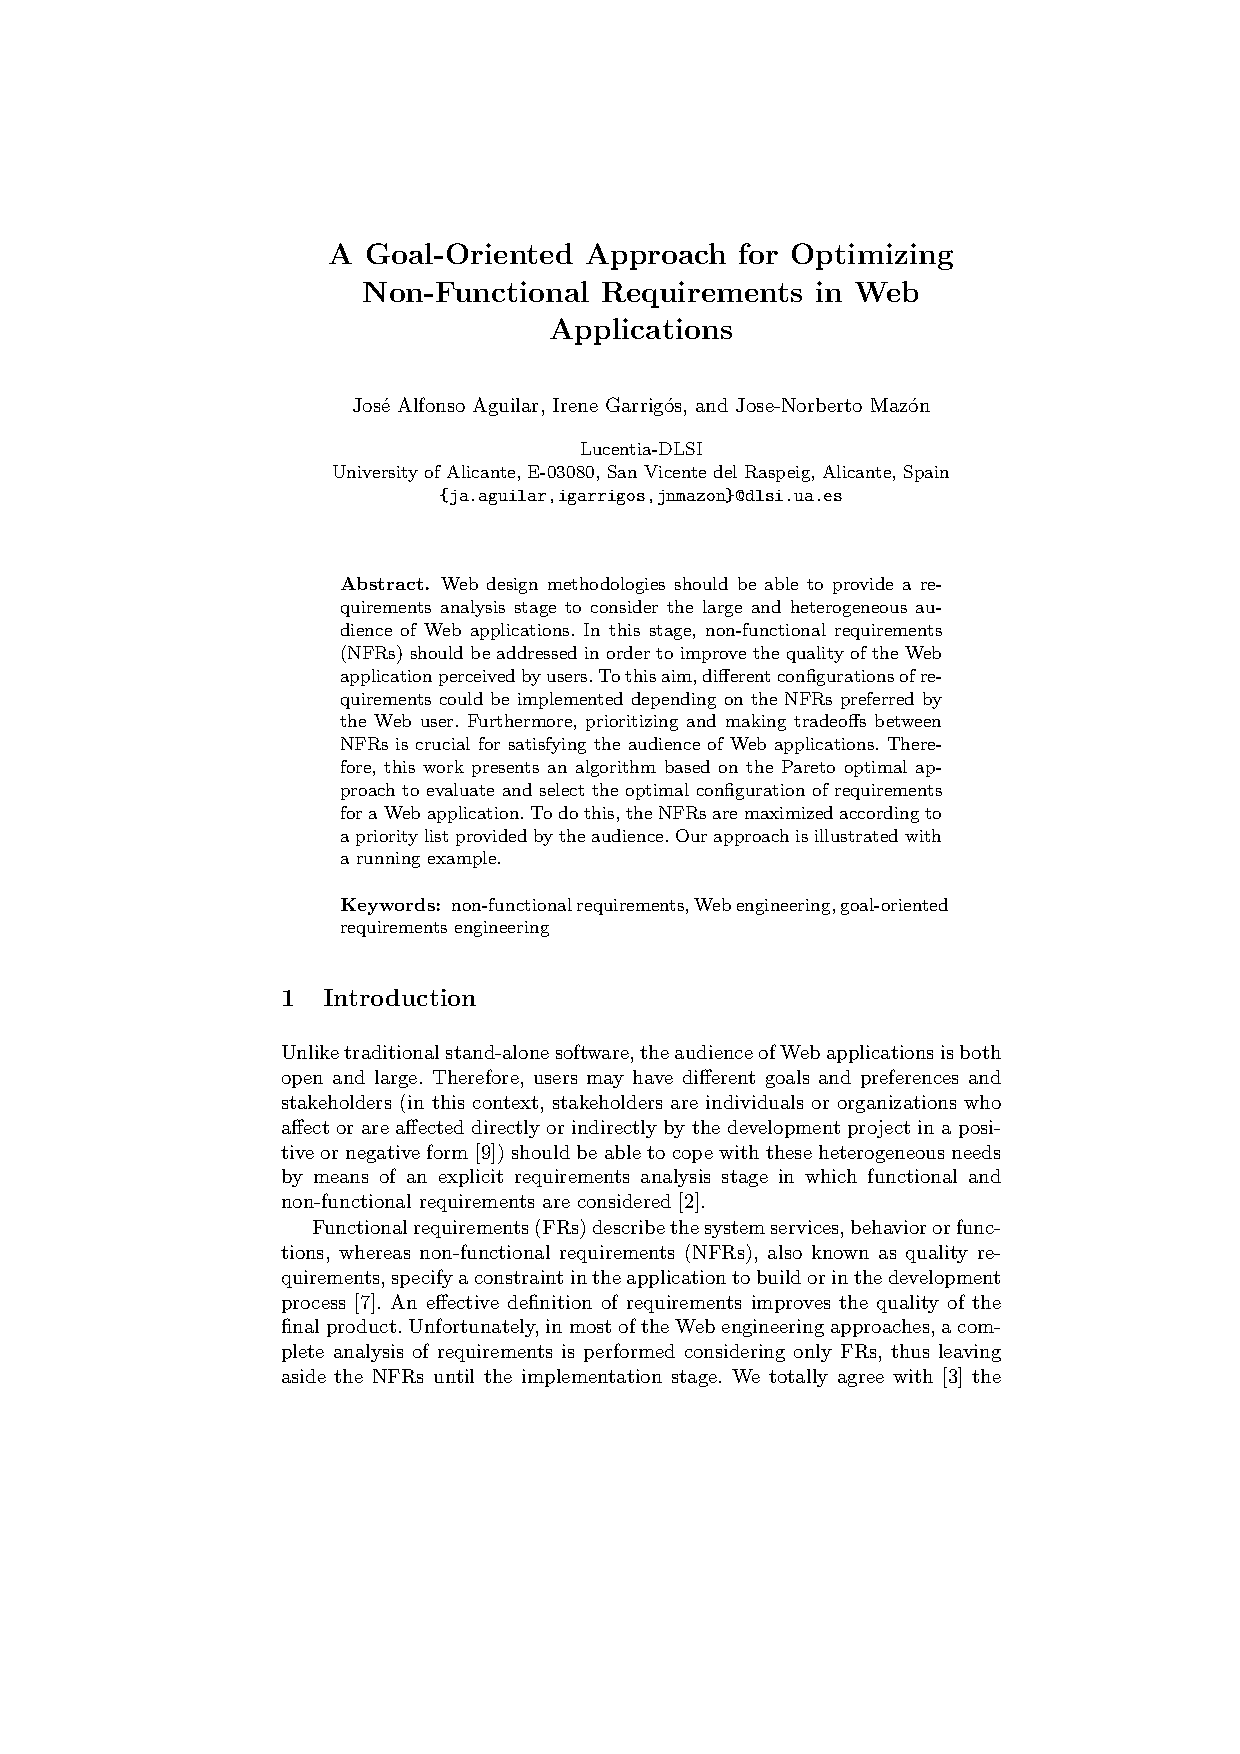
\includepdf[openright=true,pages={1-10}]{papers/AguilarWISM2011.pdf}
%
